\documentclass{beamer}
\usepackage{tikz}

\setbeamertemplate{navigation symbols}{}

\setbeamercolor{frametitle}{fg=orange}
\setbeamercolor{title}{fg=orange}
%\definecolor{tcolor}{RGB}{10,100,200}
\setbeamercolor{normal text}{fg=black}
%\setbeamercolor{normal text}{fg=RGB{} 
%\setbeamerfont{frametitle}{size=large}
\setbeamerfont{frametitle}{family=\rmfamily,shape=\itshape,size=\huge} 
\setbeamerfont{title}{family=\rmfamily,shape=\itshape,size=\huge} 

\usetheme{boxes}
\setbeamertemplate{background canvas}[vertical shading][bottom=white,top=blue!20]

\title{Cosmic Frontier at Brookhaven}

\begin{document}


%\frame{\titlepage}

\frame
{

    \frametitle{Dark Energy Survey (DES)}

    \fontsize{9}{0.8\baselineskip}

    \begin{columns}

        \begin{column}{0.5\textwidth}

            \begin{itemize}

                \item 46 DES science papers published or submitted

                \item 14 DES weak lensing papers published or submitted

                \item Weak lensing papers are based on the shear catalogs produced
                    by Erin Sheldon (BNL)

            \end{itemize}

        \end{column}

        \begin{column}{0.5\textwidth}
            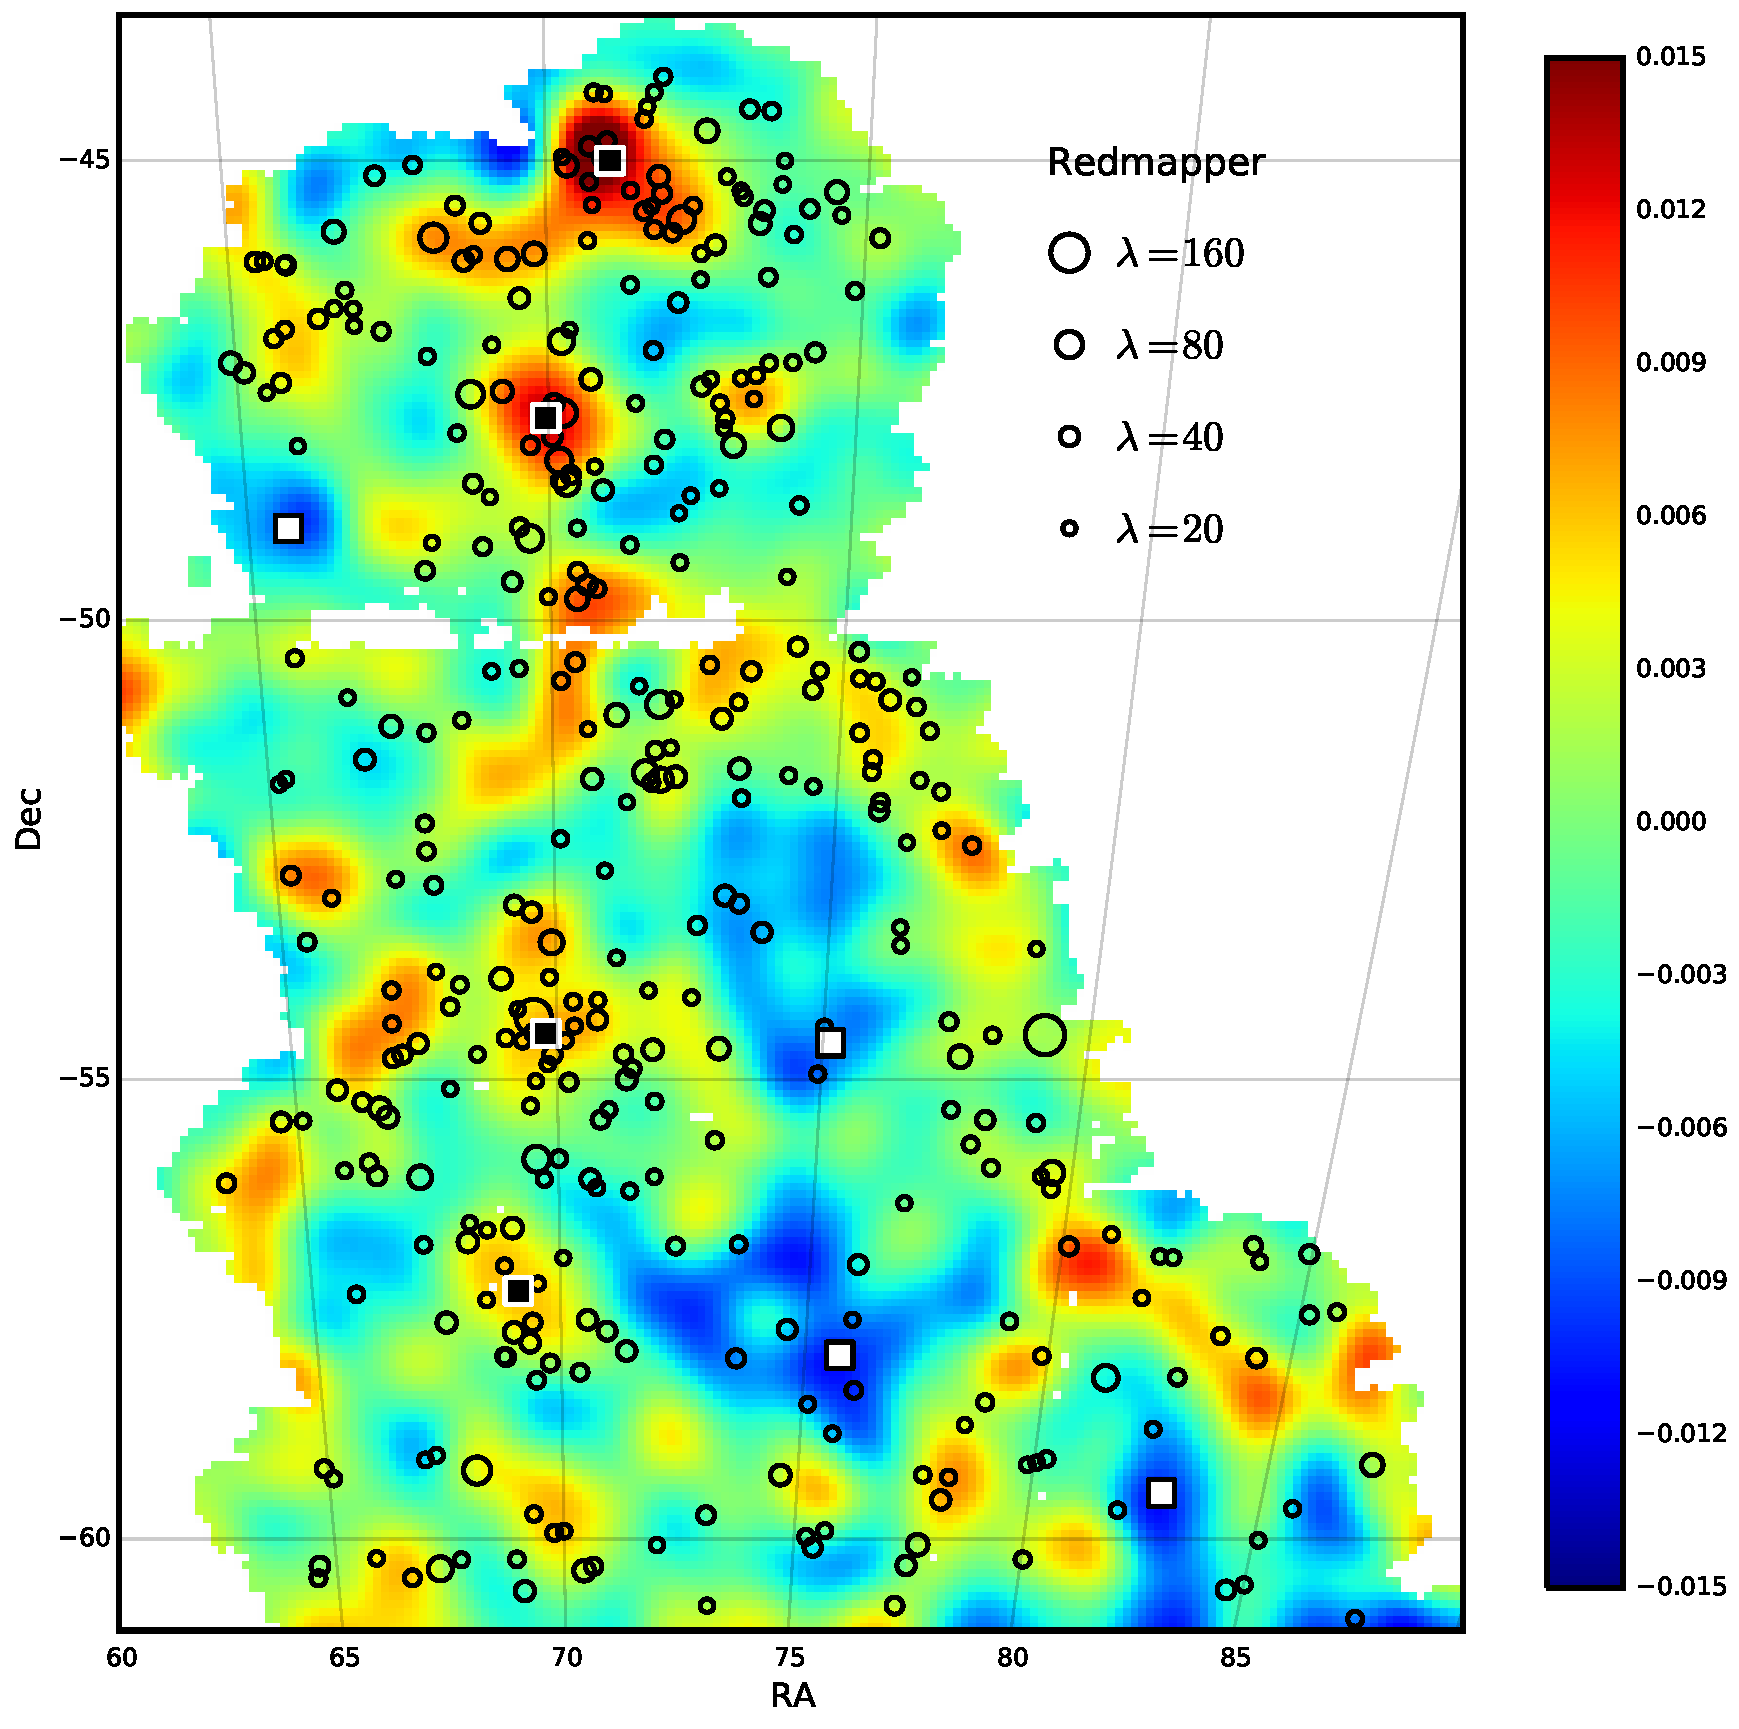
\includegraphics[scale=0.17]{cluster_overlay_ngmix_bpz.pdf}
            \newline
            {\tiny DES Mass Map, Vikram et al. 2015 PRD}
        \end{column}

    \end{columns}

}

\frame
{

    \frametitle{Dark Energy Survey}

    \fontsize{9}{0.8\baselineskip}

    \begin{columns}

        \begin{column}{0.5\textwidth}

            \begin{itemize}

                \item Sheldon was co-lead author, with Mike Jarvis, of the DES shear catalog
                    paper, as well as producing catalogs (Jarvis et al. 2016).  All
                    other lensing papers depend on this work.


                \item E. Sheldon published, with Peter Melchior, a paper on the crowd
                    sourcing ``DES Exposure Checker'', used by DES scientists
                    to view and verify survey images (Melchior, Sheldon et al. 2015).

                \item Paper on lensing by clusters of galaxies, led by E. Sheldon,
                    now in final stages.  Part of the DES key project to constrain
                    cosmology from clusters and lensing.

            \end{itemize}

        \end{column}

        \begin{column}{0.5\textwidth}
            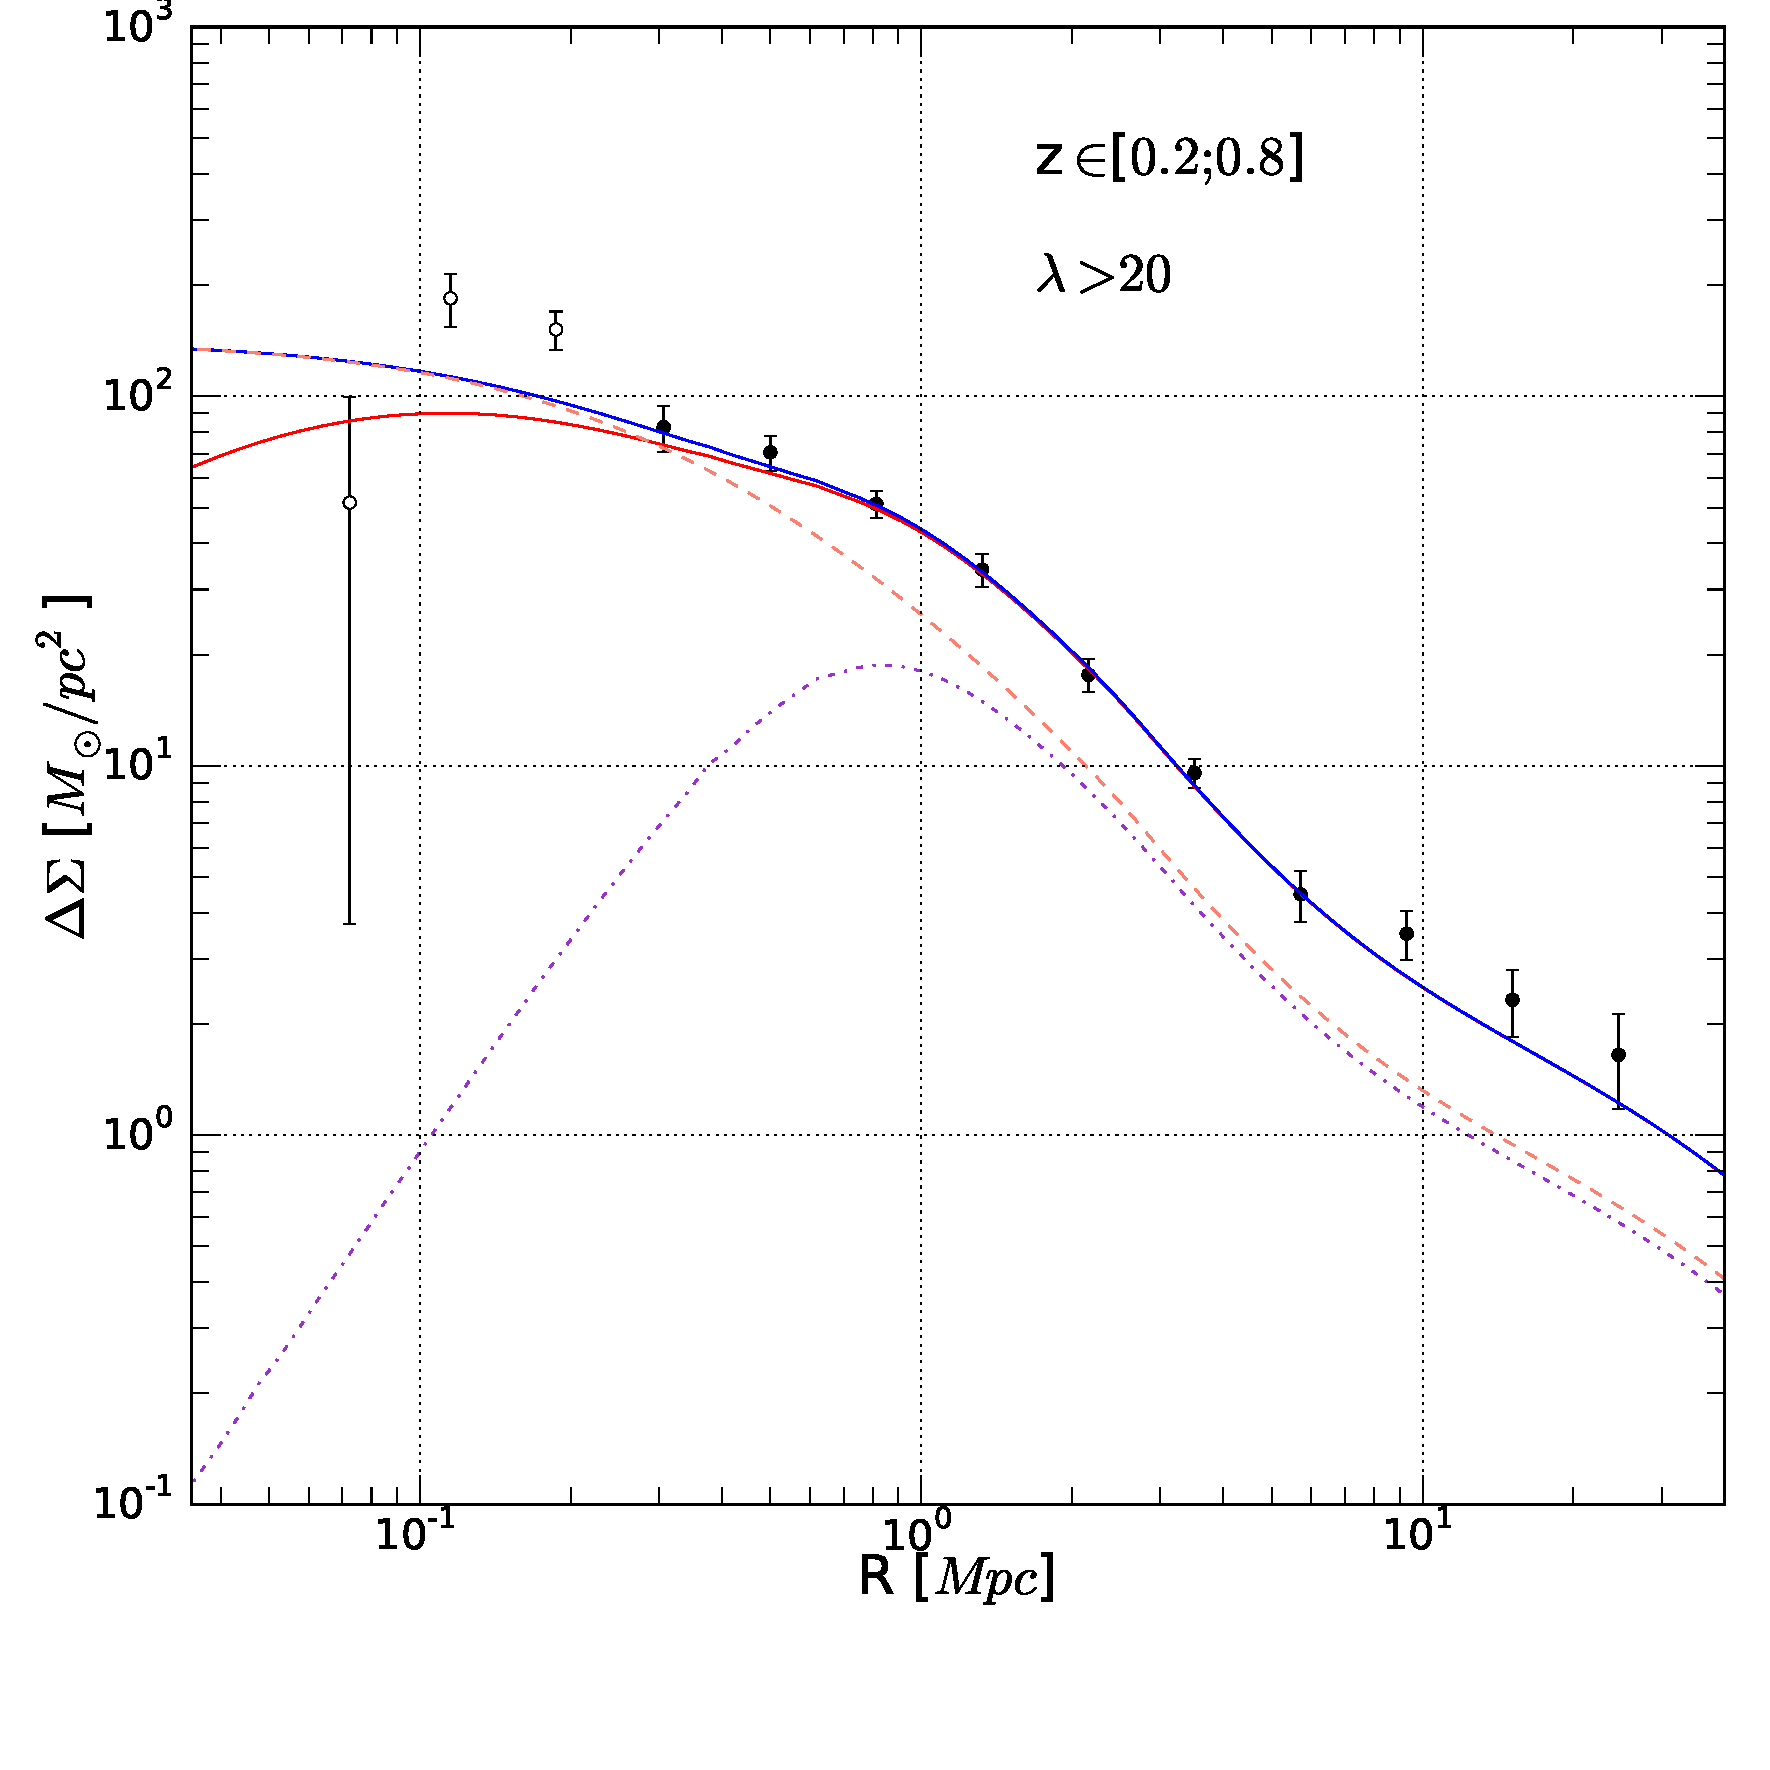
\includegraphics[scale=0.17]{delta_sigma_best_fit_z9_l9.pdf}
            \newline
            {\tiny Mass Density Constrast of DES Clusters.}
        \end{column}

    \end{columns}

}

\frame
{

    \frametitle{Dark Energy Survey}

    \fontsize{9}{0.8\baselineskip}

    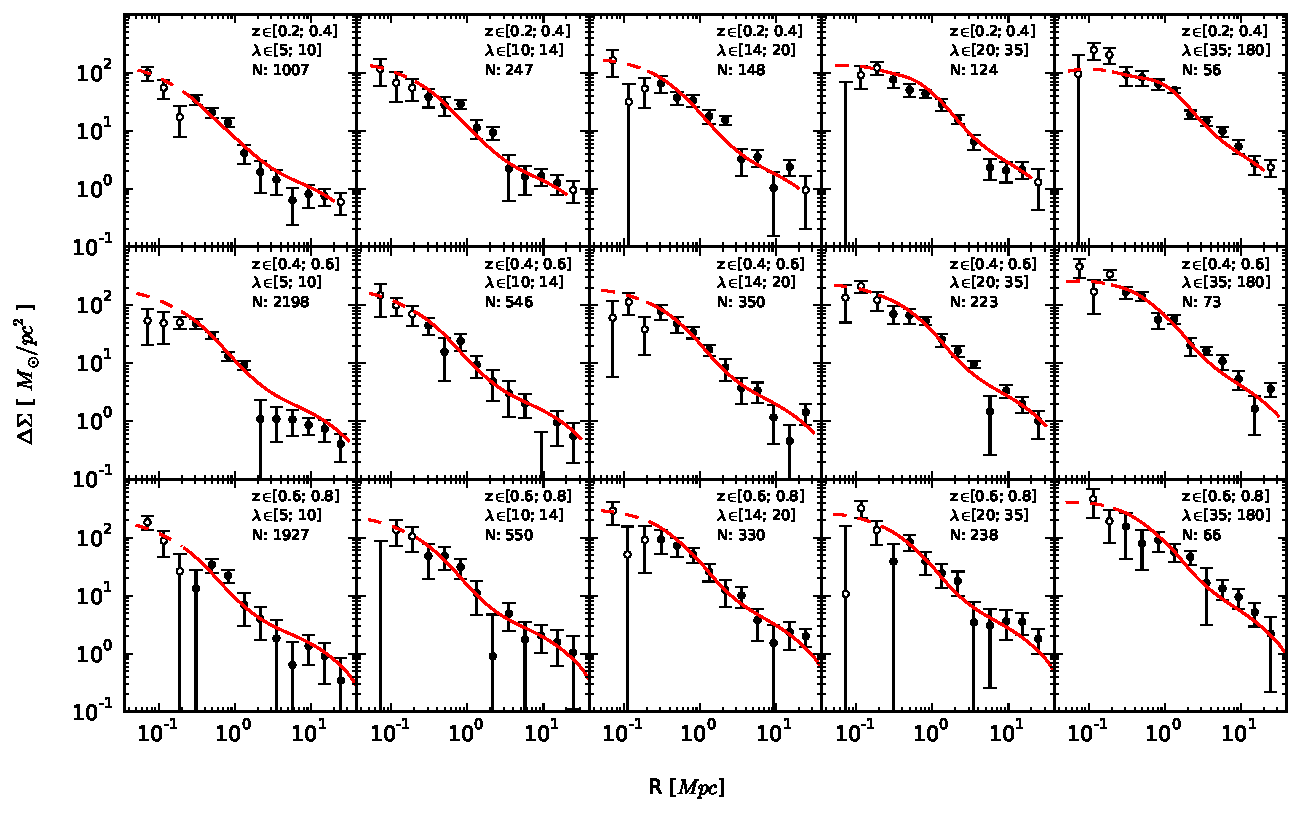
\includegraphics[width=\textwidth]{clusters-randoms_noqc_bestfit.pdf}
    \newline
    {\small Mass Density Constrast of DES Clusters as a function of richness
    and redshift.  Best fit models in red.  With more data, the redshift dependence will provide
    information about Dark Energy.}


}

\frame
{

    \frametitle{Dark Energy Survey: Ongoing and Future Work}

    \fontsize{9}{0.8\baselineskip}



            \begin{itemize}

                \item Sheldon finishing new shear pipeline.  Based on image
                    simulations, the new code appears to meet requirements for
                    DES 5 year data.

                \item New multi-object fitting code (with Matt Becker) close to
                    production-ready.  This method, measuring flux for all
                    blended objects simultaneously, is a paradigm-shift for
                    measuring fluxes in a large survey.

                \item Papers on Dark Energy will begin to appear over the next couple
                    of years.  
                    Progress has been slowed significantly due to bad weather.

            \end{itemize}


}


\frame
{

    \frametitle{Sheldon LSST Work}
    \begin{itemize}
        \item Galaxy measurement code is interesting for LSST
            \begin{itemize}

                \item An order of magnitude faster than standard codes.

                \item Can fit muliple epochs and multiple bands simultaneously.  Important
                    for LSST with very large number of epochs, many bands.

                \item Multi-object fitting nearing readiness.

            \end{itemize}

        \item Initial work to integrate code into the LSST Data Management
            code stalled due to lack of manpower in DM.

        \item Have now begun work with new postdoc in LSST (Peter Melchior) and
            integration is progressing again.

    \end{itemize}
}



\end{document}
